\chapter{Технологическая часть}

\section{Средства реализации программы}

\subsection{Выбор СУБД}

В таблице~\ref{tbl:subd}, приведена сравнительная характеристика для различных СУБД, для работы с графовой моделью данных.

\begin{table}[H]
\centering
\begin{threeparttable}
\caption{Сравнение графовых СУБД}
\begin{tabular}{|l|l|l|c|p{5cm}|}
\hline
\textbf{СУБД} & \textbf{Тип} & \textbf{Язык} & \textbf{ACID} & \textbf{Масштабируемость} \\
\hline
Neo4j         & Property Graph & Cypher        & Да   & Вертикальная, кластерная \\
\hline
OrientDB      & Multi-model    & SQL+Gremlin   & Да   & Вертикальная, кластерная \\
\hline
ArangoDB      & Multi-model    & AQL           & Да   & Горизонтальная            \\
\hline
JanusGraph    & Property Graph & Gremlin       & Частично & Горизонтальная        \\
\hline
TigerGraph    & Property Graph & GSQL          & Да   & Горизонтальная            \\
\hline
\end{tabular}
\label{tbl:subd}
\end{threeparttable}
\end{table}

В качестве СУБД была выбрана Neo4j~\cite{neo4j}, по следующим причинам:
\begin{itemize}
    \item возможность работы с графовой моделью данных напрямую, без создания дополнительных структур;
    \item активное сообщество, актуальная документация;
    \item декларативный язык Cypher, разработанный для нативной работы с графами.
\end{itemize}

Таким образом, выбор Neo4j обусловлен структурой данных задачи, необходимостью обработки иерархий и сообществ, а также производственными и удобочитаемыми преимуществами графовой модели по сравнению с реляционными СУБД.

\subsection{Выбор языка программирования}

В качестве языка программирования для реализации курсовой работы был
выбран язык C\# по следующим причинам:

\begin{itemize}
\item в стандартной библиотеке языка присутствует поддержка всех
структур данных, выбранных по результатам проектирования;
\item высокая производительность;
\item наличие официального драйвера для взаимодействия с Neo4j;
\item наличие актуальной документации.
\end{itemize}

\section{Структура ПО}

На рисунке~\ref{fig:Po struct} приведена структура разработанного ПО.

\begin{figure}[H]
	\centering
	\includegraphics[height=0.4\textheight]{Po struct.png}
	\caption{Структура ПО}
	\label{fig:Po struct}
\end{figure}

\section{Тестирование}

В таблице~\ref{tab:test-results} представлены функциональные тесты для реализации алгоритма Louvain.

\begin{table}[H]
\centering
\caption{Результаты тестирования реализации алгоритма}
\label{tab:test-results}
\begin{tabular}{|c|c|c|}
\hline
\textbf{Номер теста} & \textbf{Параметры (Inter, Intra, количество сообществ)} & \textbf{Результат} \\
\hline
1 & 0.005, 0.2, 10 & 11 \\
2 & 0.01, 0.2, 10  & 9  \\
3 & 0.05, 0.2, 10  & 8  \\
4 & 0.1,  0.2, 3  & 2  \\
5 & 0.15, 0.2, 1  & 1  \\
6 & 0.005, 0.3, 8 & 8  \\
7 & 0.01, 0.3, 10  & 7  \\
8 & 0.05, 0.3, 5  & 5  \\
9 & 0.1,  0.3, 3  & 2  \\
10 & 0.15, 0.3, 1 & 1  \\
11 & 0.005, 0.4, 5 & 5  \\
12 & 0.01, 0.4, 5 & 4  \\
13 & 0.05, 0.4, 5 & 3  \\
14 & 0.1,  0.4, 3 & 1  \\
15 & 0.15, 0.4, 3 & 1  \\
16 & 0.005, 0.5, 3 & 3  \\
17 & 0.01, 0.5, 2 & 2  \\
18 & 0.05, 0.5, 2 & 2  \\
19 & 0.1,  0.5, 1 & 1  \\
20 & 0.15, 0.5, 1 & 1  \\
21 & 0.005, 0.6, 2 & 2  \\
22 & 0.01, 0.6, 5 & 5  \\
23 & 0.05, 0.6, 1 & 1  \\
24 & 0.1,  0.6, 1 & 1  \\
25 & 0.15, 0.6, 1 & 1  \\
\hline
\end{tabular}
\end{table}

\section{Визуализация данных}

Для демонстрации данных был выбран стандартный браузер Neo4j. На рисунке~\ref{fig:data} приведён пример визуализации данных.

\begin{figure}[H]
	\centering
	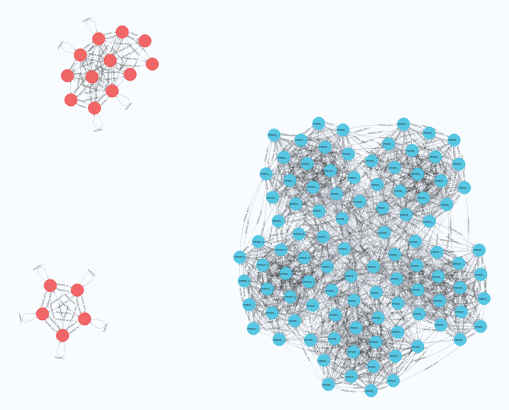
\includegraphics[height=0.4\textheight]{data.png}
	\caption{Пример визуализации данных}
	\label{fig:data}
\end{figure}

\section*{Вывод}

В технологической части был обоснован выбор средств реализации программного обеспечения. В качестве базы данных использована графовая СУБД Neo4j, которая наиболее полно отражает природу предметной области, связанную с моделированием социальных графов и иерархических структур сообществ. Её язык запросов Cypher и встроенная поддержка работы с графами позволили упростить реализацию операций над данными.

Для разработки программной логики выбран язык C\#~\cite{Csharp}, обеспечивающий высокую производительность, удобную работу с асинхронностью и наличие официальной поддержки драйвера для Neo4j. 

Визуализация структуры графа и результатов работы алгоритма осуществляется средствами встроенного браузера Neo4j, что позволило наглядно продемонстрировать полученные данные без необходимости использования сторонних решений.

Выбор указанных технологий обеспечил удобство, надёжность и расширяемость при реализации поставленной задачи.

